\chapter{HELIUM ISO-SEQUENCE}
% !TEX root = hazy3.tex

\section{Overview}

The helium-like isoelectronic sequence is treated with a single unified
approach that was developed by Ryan Porter as his PhD thesis.  These are
published in \citet{Bauman2005}, \citet{Porter2005}, Porter et al.
(2007), and \citet{PorterFerland2007}

\section{Energy levels}

Figure \ref{fig:helium_energy_levels} shows a partial
Grotrian diagram for He-like ions.
The order of the $J$ levels within $2p\;{P^o}$
is reversed for the atom; the energy levels shown in
Figure \ref{fig:helium_energy_levels} are for
astrophysically abundant ions.  In the code the energies associated with
a particular $J$ level are always correct, but for He I these occur out of
order in the vector of energy levels.  This is ok since the levels are so
close to having the same energy.

\begin{figure}
\centering
\label{fig:helium_energy_levels}
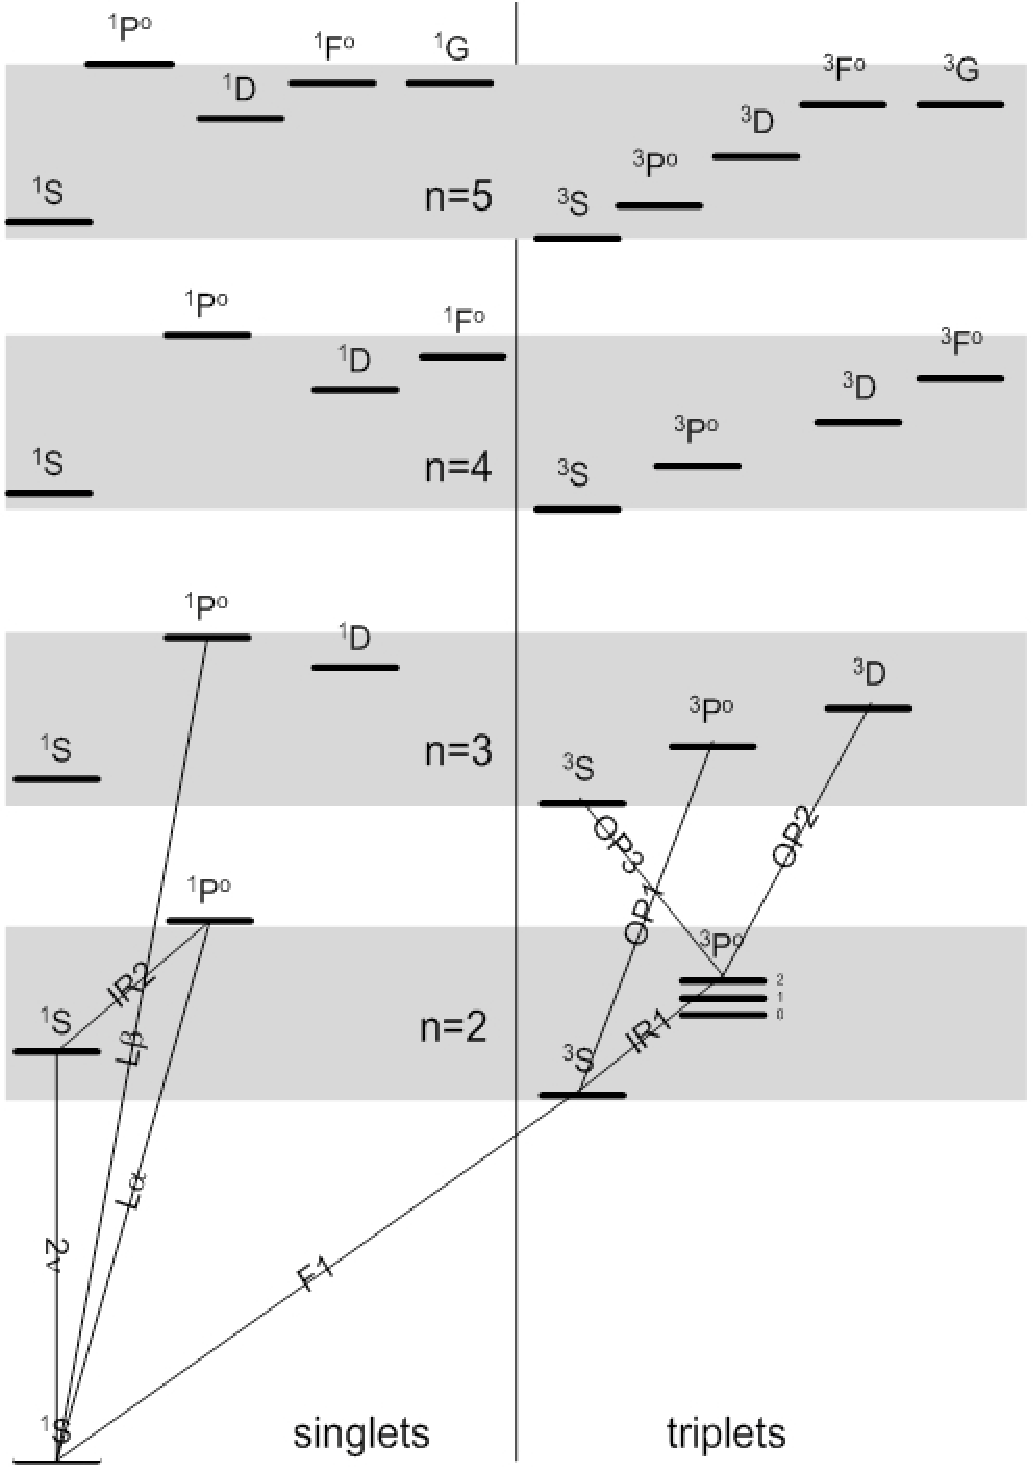
\includegraphics[scale=0.7]{helium_energy_levels}
\caption[He iso sequence energy levels]{A partial Grotrian diagram for the helium iso-electronic sequence.}
%helium
\end{figure}


Figure \ref{fig:HeEnergiesHighNLevel} compares the energies of the levels within a high-n complex
of \hei.  For comparison, the equivalent hydrogenic energies is drawn as
a dotted line.  The $^1P$ level is actually above the hydrogenic level but
all other \hei\ levels are below, and their energies approach the hydrogen
case as the angular momentum increases.  Singlets always have higher energies
than triplets.

\begin{figure}
\label{fig:HeEnergiesHighNLevel}
\centering
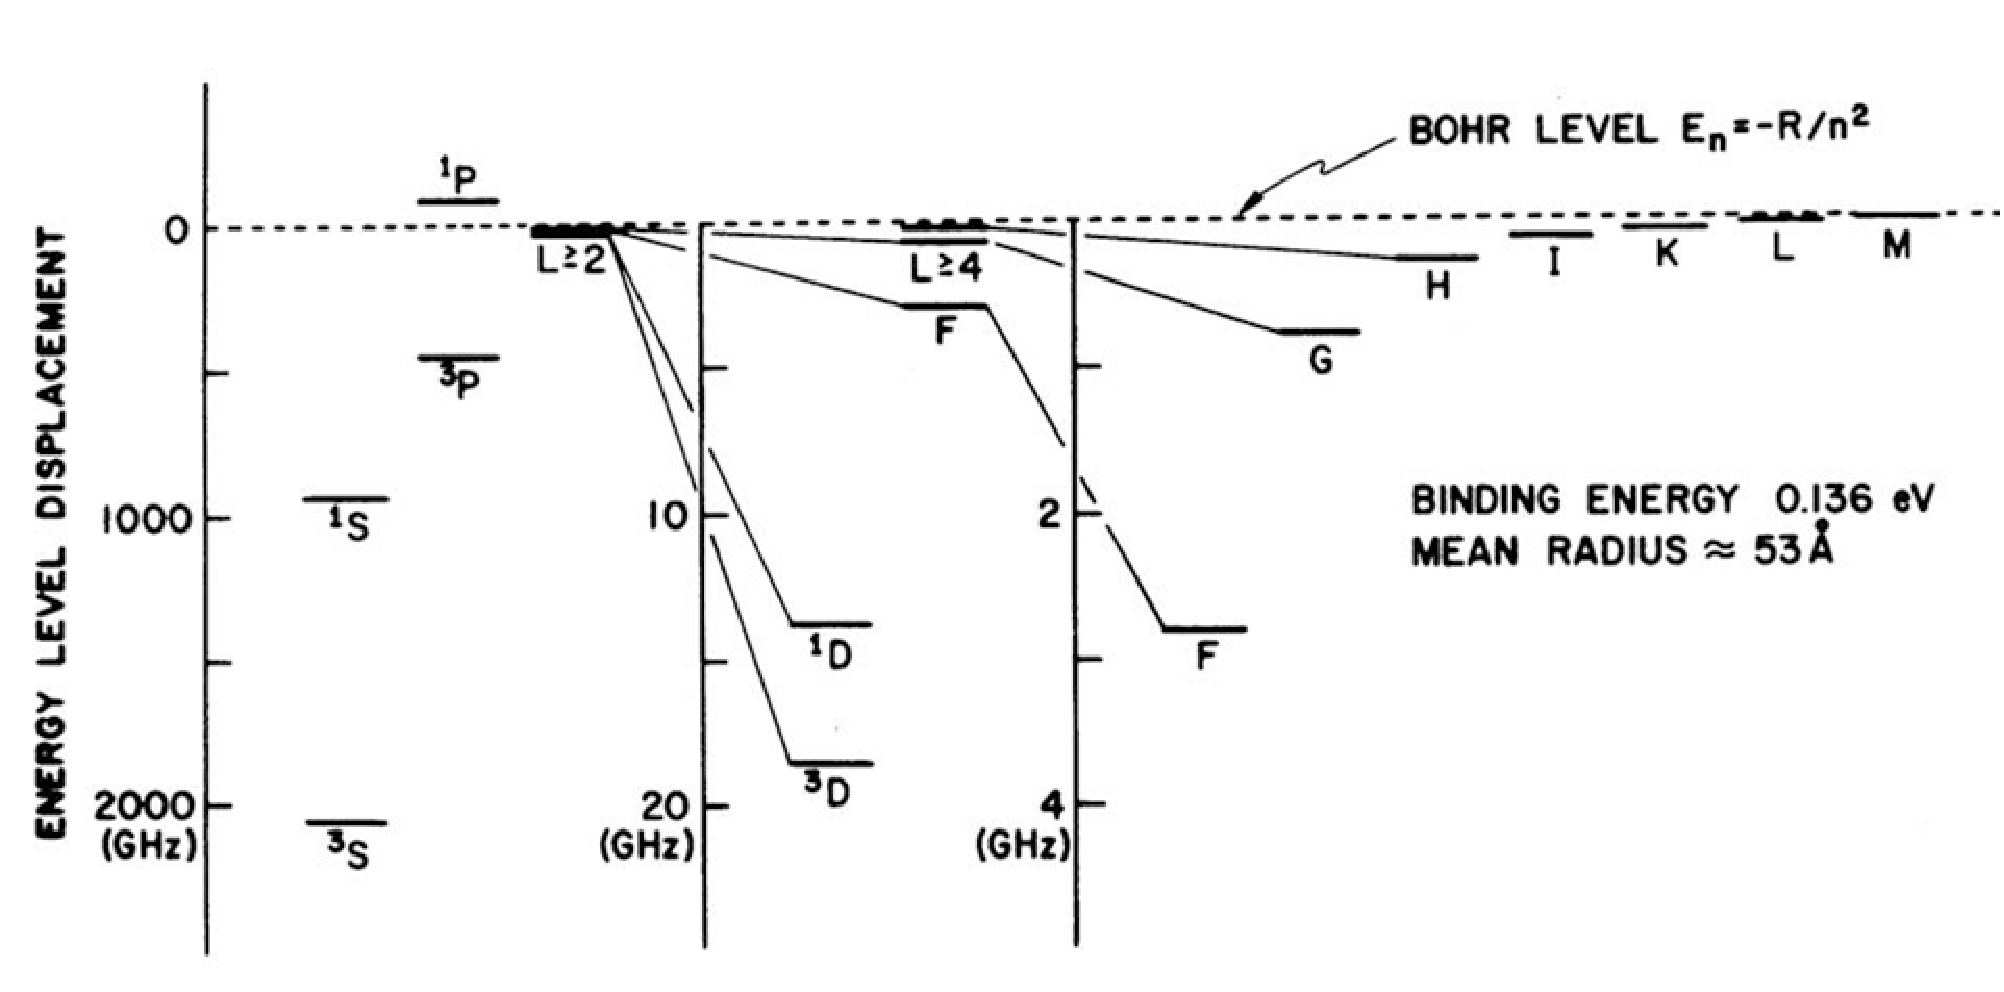
\includegraphics[scale=0.5]{HeEnergiesHighNLevel}
\caption[Energies within high-n levels of He]{A  comparison of energies of various states within a high-$n$ state
of He0.  From Wing \& McAdam (1978).}
\end{figure}

Wavelengths for lines coming from the $n = 2$ complex are listed in
Table~\ref{tab:HeLikeWavelengths}

\begin{table}
\label{tab:HeLikeWavelengths}
\caption{Wavelengths of transitions of the He-like sequence}
\begin{tabular}{lllllllll}
\hline
Z& Elem& 2 $^1$P-1 $^1$S& 2 $^3$P1-1 $^1$S& 2 $^3$P2-1 $^1$S& 2 $^3$S-1
$^1$S& 2 $^3$P$_2$-2 $^3$S& 2 $^3$P$_1$-2 $^3$S& 2 $^3$P$_0$-2 $^3$S\\
\hline
2&He& 584.3A& 591.4A& 591.4A& 625.6A& 1.083m& 1.083m& 1.083m\\
3& Li& 199.3A& 202.3A& 202.3A& 210.1A&
5484A& 5485A& 5483A\\
4& Be& 100.3A& 101.7A& 101.7A& 104.5A& 3721A& 3723A& 3721A\\
5& B&
60.31A& 61.09A& 61.09A& 62.44A& 2822A& 2826A& 2825A\\
6& C& 40.27A& 40.73A& 40.73A& 41.47A& 2271A&
2278A& 2277A\\
7& N& 28.79A& 29.08A& 29.08A& 29.53A& 1897A& 1907A& 1908A\\
8& O&
21.60A& 21.81A& 21.80A& 22.10A& 1624A& 1638A& 1640A\\
9& F& 16.81A& 16.95A& 16.94A& 17.15A& 1395A&
1414A& 1417A\\
10& Ne& 13.45A& 13.55A& 13.55A& 13.70A& 1248A& 1273A&
1278A\\
11& Na& 11.00A& 11.08A& 11.08A& 11.19A& 1112A& 1142A&
1149A\\
12& Mg& 9.169A& 9.231A& 9.228A& 9.314A& 997.5A& 1034A&
1043A\\
13& Al& 7.757A& 7.807A&7.804A& 7.872A& 899.7A& 943.2A& 954.3A\\
14& Si& 6.648A& 6.688A& 6.685A& 6.740A& 814.7A& 865.1A& 878.6A\\
15& P& 5.760A& 5.793A& 5.790A& 5.836A& 740.0A& 797.5A& 813.2A\\
16& S& 5.039A& 5.066A& 5.063A& 5.102A& 673.4A& 738.3A& 756.3A\\
17& Cl& 4.444A& 4.468A& 4.464A& 4.497A& 613.8A& 686.1A& 706.0A\\
18& Ar& 3.949A& 3.969A& 3.966A& 3.994A& 560.0A& 639.6A& 661.6A\\
19& K& 3.532A& 3.550A& 3.546A& 3.571A& 510.7A& 596.3A& 621.5A\\
20& Ca& 3.177A& 3.193A& 3.189A& 3.211A& 466.9A& 560.7A& 585.9A\\
21& Sc& 2.873A& 2.887A& 2.883A& 2.903A& 426.1A& 525.1A& 553.6A\\
22&Ti& 2.610A& 2.623A& 2.619A& 2.637A& 389.5A& 496.6A& 523.9A\\
23&V& 2.382A& 2.393A& 2.389A& 2.406A& 355.8A& 469.0A& 496.9A\\
24&Cr& 2.182A& 2.193A& 2.189A& 2.203A& 325.0A& 444.0A& 472.1A\\
25& Mn& 2.006A& 2.016A& 2.012A& 2.026A& 296.8A& 421.1A& 449.3A\\
26& Fe& 1.850A& 1.860A& 1.855A& 1.868A& 271.2A& 400.3A& 428.2A\\
27& Co& 1.712A& 1.721A& 1.716A& 1.728A& 247.6A& 381.2A& 408.6A\\
28& Ni& 1.588A& 1.597A& 1.592A& 1.604A& 226.3A& 363.9A& 390.5A\\
29& Cu& 1.478A& 1.485A& 1.481A& 1.492A& 206.7A& 347.7A& 373.5A\\
30& Zn& 1.378A& 1.385A& 1.381A& 1.391A& 188.9A& 333.0A& 357.3A\\
\hline
\end{tabular}
\end{table}


\section{The He I triplets}

   The population of the metastable 2s $^3$S level is determined including
all processes that create and destroy the level.  Processes that destroy
2s 3S include photoionization and collisional ionization, radiative decays
to ground, and collisional transitions to the singlets.  Processes that
create populations include three-body and radiative recombination and
collisions to the triplets from the singlets.  Including only radiative
recombination, exchange collisions to the singlets, and radiative decays
to ground, the relative population of the 2$^3$S level of He$^0$ can be written
as
\begin{equation}
\frac{{He({2^3}S)}}{{H{e^ + }}} = \frac{{5.79 \times {{10}^{ - 6}}\;t_4^{
- 1.18}}}{{1 + 3110\,t_4^{ - 0.51}n_e^{ - 1}}}
\end{equation}
where $t_4$ is the electron temperature in units of 10$^4$~K.

\section{Collapsed versus resolved levels}

A level in which all of the spin and angular momentum states are
explicitly determined individually is said to be resolved.  One in which
these are replaced by a single level, with the sublevels assumed to be
populated according to their statistical weight, is said to be collapsed.
Treating a level as a collapsed levels saves computer time and is appropriate
if the density is high enough for collisions to make the state fully l-mixed.

Figure \ref{fig:l_mixed_pengelly_seaton} shows a plot of the density needed to $l$-mix a level (the y-axis)
vs the principle quantum number (the x-axis).  The data are taken from
\citet{PengellySeaton1964}.
This can be used as a guide for adjusting what
levels can be treated as the collapsed case.

\begin{figure}
\centering
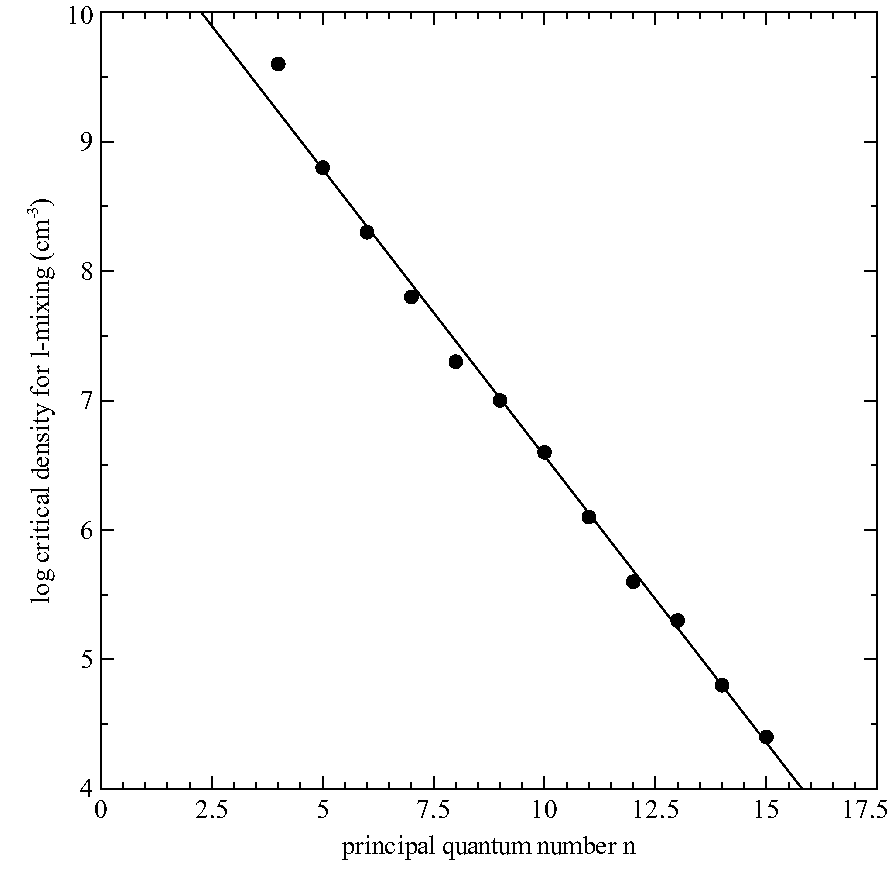
\includegraphics{l_mixed_pengelly_seaton}
\label{fig:l_mixed_pengelly_seaton}
\caption[l-mixed principle quantum number vs density]
{The lowest principle quantum number which can be treated as $l$-mixed
(the x-axis) is shown versus the density for this to occur (the y-axis).
Original data taken from \citet{PengellySeaton1964}.}
\end{figure}

\section{Emission from a pure helium gas}

Figure \ref{fig:HeI_emission} shows the predicted line and continuous
emission for a pure helium gas.

\begin{figure}
\label{fig:HeI_emission}
\centering
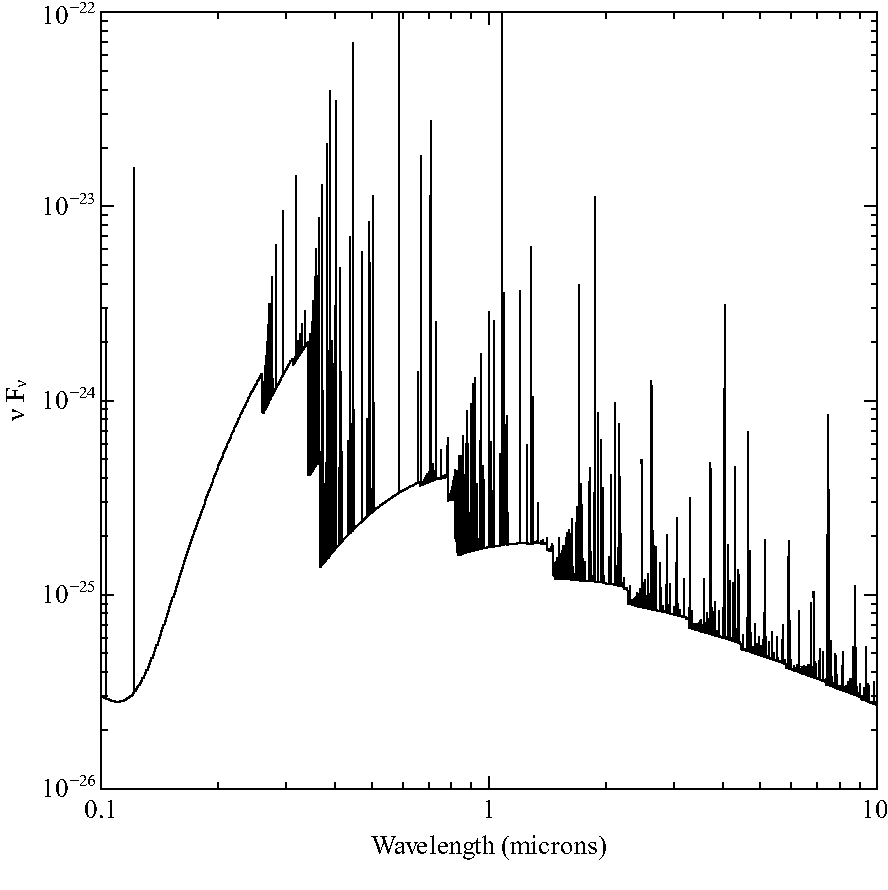
\includegraphics{HeI_emission}
\caption[He I emission]
{The net emission from a pure atomic helium gas at $10^4 \K$.  This
is from the calculation \cdFilename{heatomt10.in}
in the test suite.}
\end{figure}
